\documentclass[11pt]{article}
\usepackage{acl}
\usepackage{times}
\usepackage{latexsym}
\usepackage[T1]{fontenc}
\usepackage[utf8]{inputenc}
\usepackage{microtype}
\usepackage{amsmath,amssymb}
\usepackage{graphicx}
\usepackage{booktabs}
\usepackage{multirow}
\usepackage{url}
\title{Character- and Shape-Aware BiLSTM POS Tagging Under a 100-Dimensional Representation Budget}
\author{\textbf{Yash Gupta}\\Roll No.: \texttt{23118081}\\Department of Data Science and Artificial Intelligence, IIT Roorkee \And \textbf{Adarsh Maurya}\\Roll No.: \texttt{23125004}\\Department of Data Science and Artificial Intelligence, IIT Roorkee}
\date{}
\begin{document}
\maketitle
\begin{abstract}
We study a lightweight neural part-of-speech (POS) tagger under the DAL-585 PA2 constraints: no pretrained word vectors and at most 100 dimensions in the input token representation. The selected system combines a trainable lexical embedding, a multi-width character CNN, and an orthographic-shape embedding, followed by a two-layer bidirectional LSTM and token-level softmax. Selection uses a deterministic 5\% sentence holdout from the training corpus; the supplied development labels are kept out of model selection. Across 23 single-seed experiments, label-smoothed training gives the highest internal validation accuracy (97.585\%). After refitting on the full training set, the model reaches 97.739\% token accuracy and 89.803\% exact-surface out-of-vocabulary accuracy on 47,633 development tokens. Error analysis highlights noun--adjective, adposition--adverb/particle, and verb-form confusions. We compare against Yash Gupta's PA1 bigram HMM, which obtained 96.4122% development accuracy; Adarsh Maurya's independently built HMM result remains pending until its measured score is available.
\end{abstract}

\section{Introduction}
Part-of-speech tagging assigns each token a grammatical category. Frequent lexical items can often be identified from their learned word vectors, but ambiguous forms such as \emph{chief}, \emph{kind}, and participles require context; unseen surface forms additionally benefit from orthographic and morphological evidence. The Penn Treebank (PTB) provides the fine-grained tag inventory used here \citep{marcus1993}. A tuned bigram HMM provides a statistical baseline; TnT's unknown-word treatment motivates capitalization and suffix evidence for rare tokens \citep{brants2000}.

Neural POS taggers have combined lexical embeddings with character-level representations to encode morphology and spelling \citep{santos2014}. Bidirectional LSTMs contextualize a token using both its left and right context, while a CRF can model dependencies across output labels \citep{huang2015,mahovy2016}. Our goal is not to use a pretrained language model: PA2 explicitly prohibits pretrained word vectors. Instead, we compare compact trainable representations and sequence encoders under the 100-D input budget.

We make three practical contributions. First, we report a reproducible, training-derived validation protocol and 23 controlled architecture/optimization variants. Second, we measure how lexical, character, shape, directionality, decoder, and regularization choices affect validation and OOV accuracy. Third, we analyze the final model on the provided development set and compare aggregate metrics with Yash's PA1 bigram HMM; Adarsh's independent HMM result remains pending.

\section{Data and Vocabulary}
The training corpus contains 39,832 tagged sentences (950,028 tokens) and 45 POS labels. We deterministically shuffle sentence indices with seed 42 and reserve 5\% (1,992 sentences, 47,323 tokens) for selection; the remaining 37,840 sentences are used to fit the 23 variants. The separate development corpus has 1,993 sentences and 47,633 gold-tagged tokens. It contains 44 distinct gold labels; the tag \texttt{SYM} appears in training but not in development. Development labels are used only after model selection and final refitting.

Lexical keys are lowercased and digits are mapped to \texttt{0}; the final training vocabulary contains 34,553 normalized lexical types (34,555 IDs including padding and unknown entries). Character encoding preserves original spelling, adds boundary markers, and truncates long tokens by retaining a prefix and suffix. Characters seen fewer than twice share an unknown-character ID. Eight deterministic surface-shape classes represent capitalization, digits, punctuation-only forms, hyphens, and mixed forms. At inference, an unseen lexical key maps to the unknown word embedding but still receives character and shape features; no pretrained vectors are loaded.

\section{Model Architecture}
For token $w_t$, the selected model forms a lexical vector $e_t^w\in\mathbb{R}^{50}$, a character representation $e_t^c\in\mathbb{R}^{40}$, and a learned shape vector $e_t^s\in\mathbb{R}^{10}$. The input is
\begin{equation}
 x_t=[e_t^w;e_t^c;e_t^s]\in\mathbb{R}^{100}.
\end{equation}
The character encoder embeds characters in 25 dimensions and applies two convolution banks of widths 3 and 5 (20 filters per width), followed by masked max pooling and concatenation. This allows short suffixes/prefixes and slightly longer spelling patterns to contribute features without exceeding the dimensionality budget.

The sequence $(x_1,\ldots,x_T)$ passes through a two-layer BiLSTM with 256 hidden units in each direction. Its top-layer state $h_t=[\overrightarrow h_t;\overleftarrow h_t]\in\mathbb{R}^{512}$ is projected to 45 logits, and the prediction is
\begin{equation}
 p(y_t=k\mid w_{1:T})=\operatorname{softmax}(Wh_t+b)_k.
\end{equation}
The selected model uses a per-token softmax rather than a CRF. Figure~\ref{fig:arch} summarizes the complete path from the input token to its tag.

\begin{figure*}[t]
\centering
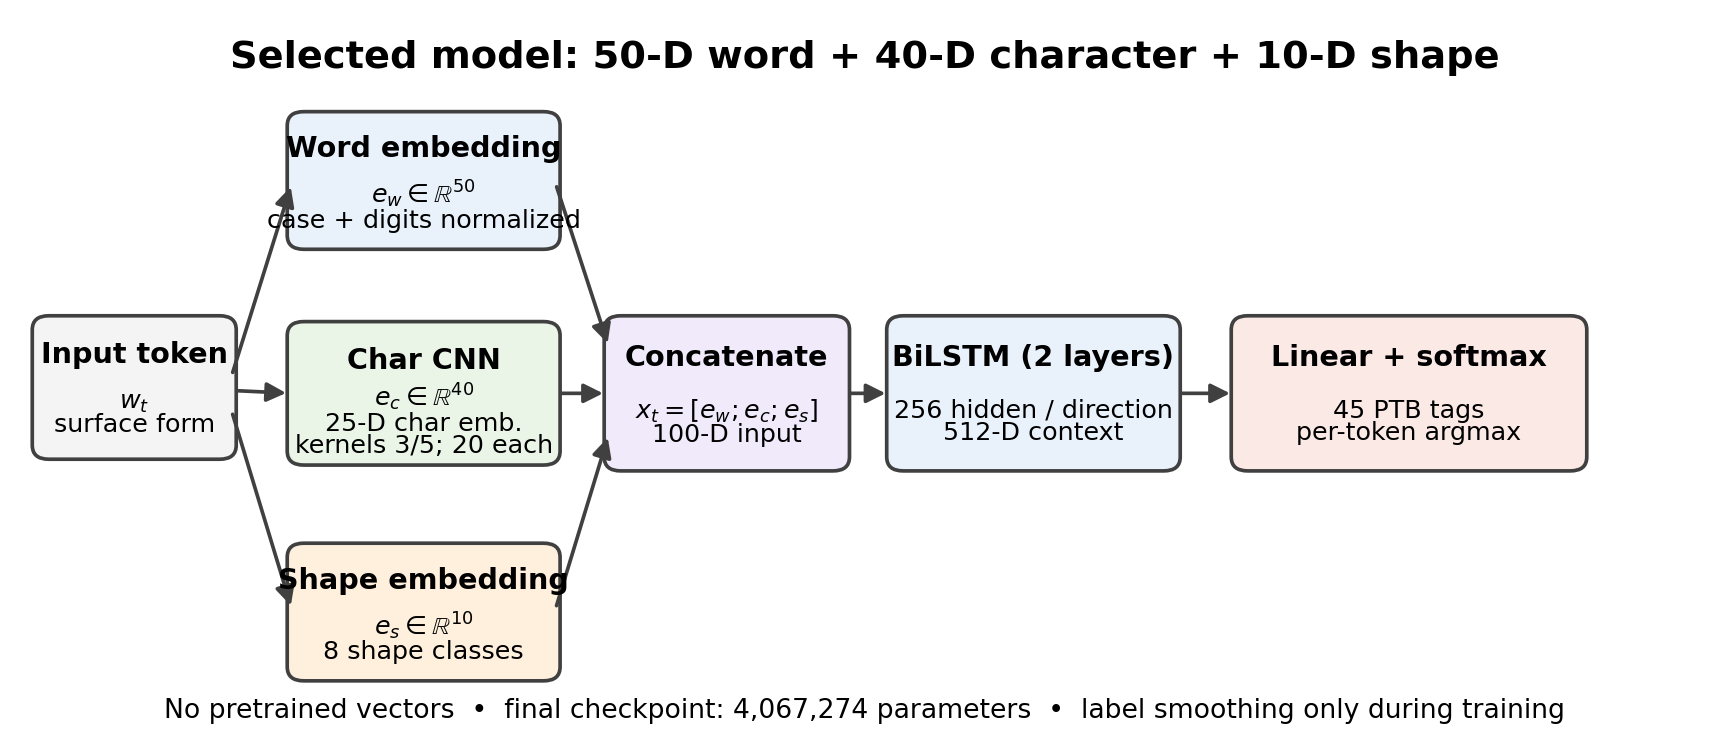
\includegraphics[width=0.98\textwidth]{figures/architecture.png}
\caption{Selected character- and shape-aware tagger. The concatenated token input is exactly 100-D; the contextual BiLSTM state is 512-D. Embeddings are trained from scratch.}
\label{fig:arch}
\end{figure*}

\section{Training Algorithms, Loss Functions, and Experimental Setup}
For the softmax variants, we minimize token-level cross-entropy with label smoothing $\epsilon=0.1$ in the selected configuration. For gold label $y_t$ and $K=45$ tags, the smoothed target distribution is $q_{t,k}=(1-\epsilon)\mathbb{1}[k=y_t]+\epsilon/K$ and
\begin{equation}
 \mathcal{L}=-\frac{1}{N}\sum_{t=1}^{N}\sum_{k=1}^{K}q_{t,k}\log p_{t,k},
\end{equation}
where $N$ counts non-padding tokens. Optimization uses AdamW (learning rate 0.002, weight decay $10^{-5}$), batches of 96 sentences, global gradient clipping at 5, input/output dropout 0.35, inter-layer LSTM dropout 0.25, and frequency-aware word dropout with $p_{\mathrm{drop}}(w)=\alpha/(\alpha+c(w))$ for $\alpha=1$. Dropping the word ID leaves character and shape features available. A validation-loss scheduler halves the learning rate on a plateau; early stopping selects the best validation-accuracy checkpoint with patience 4 and minimum change $3\times10^{-5}$.

All 23 variants use seed 42 and the same fixed sentence-level validation split. They cover word-only and word+shape inputs, character CNN and character LSTM encoders, case-sensitive lookup, unidirectional recurrence, CRF versus softmax decoding, several 100-D allocations, LSTM depth/width, dropout, word dropout, learning rate, batch size, and label smoothing. The highest validation score selects the configuration; it is then refit for 16 epochs on all 39,832 training sentences. This two-stage procedure uses the development labels only for final evaluation, not tuning.

\section{Results and Ablations}
Table~\ref{tab:ablations} gives representative controlled comparisons from the training-derived validation set. Replacing a word-only 100-D lookup representation with a 60-D word + 40-D character representation raises validation accuracy from 96.313\% to 97.492\% and exact-surface OOV accuracy from 70.52\% to 88.26\%. Moving from that 60/40 allocation to 50/40/10 (word/character/shape) raises accuracy by another 0.042 percentage points; because this reallocates ten dimensions from word to shape, it is not an isolated shape-only effect. The dimension-allocation tests compare designs under a fixed 100-D budget, and are not all strict one-factor interventions. Replacing the BiLSTM with a forward-only LSTM reduces accuracy by 0.862 percentage points. Character CNN and character LSTM are virtually tied in accuracy, but the character LSTM run takes about 179 s versus 139 s for the CNN run. The CRF variant reaches 97.559\%, just 0.025 percentage points above the same-encoder softmax baseline at 97.534\%, while taking about 2.66 times as long. These small gaps are not robust evidence of superiority because each variant was run with one seed.

\begin{table*}[t]
\centering
\small
\setlength{\tabcolsep}{5pt}
\begin{tabular}{p{5.1cm}rrrr}
\toprule
Variant (word/char/shape D) & Val. acc. & Surface OOV & Params. (M) & Time (s)\\
\midrule
Word only (100/0/0) & 96.313 & 70.52 & 5.709 & 128.4\\
Word + shape (90/0/10) & 97.073 & 77.30 & 5.372 & 139.7\\
Word + character CNN (60/40/0) & 97.492 & 88.26 & 4.365 & 145.7\\
Full CNN + BiLSTM + softmax (50/40/10) & 97.534 & 89.65 & 4.028 & 139.4\\
Forward-only LSTM (50/40/10) & 96.672 & 86.00 & 2.599 & 103.8\\
Character LSTM + BiLSTM (50/40/10) & 97.532 & 89.13 & 4.031 & 179.0\\
Full CNN + CRF (50/40/10) & 97.559 & 89.57 & 4.030 & 370.6\\
Peer-report-like variant (80/20/0) & 97.452 & 87.22 & 4.060 & 141.1\\
Label smoothing $\epsilon=0.1$ (50/40/10, selected) & 97.585 & 88.00 & 4.028 & 153.0\\
\bottomrule
\end{tabular}
\caption{Validation accuracy and exact-surface OOV accuracy on the same 47,323-token holdout. Parameters and times are for the split-trained models. Single seed; differences below a few tenths of a point require replication.}
\label{tab:ablations}
\end{table*}

On the separate development set, the full-data model correctly tags 46,556 of 47,633 tokens (97.739\%). Exact-sentence accuracy is 60.863\% (1,213/1,993). Exact-surface OOV accuracy is 89.803\% (1,092/1,216); after lowercasing and digit normalization, 867 tokens remain lexically OOV and accuracy on this subset is 88.120\%. The final model has 4,067,274 trainable parameters. Full sweep time was 61.1 minutes, the final refit took 132.6 s for 16 epochs, and the measured \texttt{run\_tagger.py} process including model loading took 5.36 s for the development input.

\begin{table*}[t]
\centering
\small
\setlength{\tabcolsep}{3pt}
\begin{tabular}{p{2.8cm}p{3.2cm}p{2.7cm}p{6.0cm}}
\toprule
\textbf{Evaluation metric} & \textbf{Score} & \textbf{Training/runtime} & \textbf{Value}\\
\midrule
Dev token accuracy & 97.739\% (46,556/47,633) & Token input & 50-D word + 40-D char + 10-D shape = 100-D\\
Exact-sentence accuracy & 60.863\% (1,213/1,993) & Optimizer / learning rate & AdamW / 0.002\\
Exact-surface OOV & 89.803\% (1,092/1,216) & Batch / final epochs & 96 sentences / 16 epochs\\
Normalized lookup OOV & 88.120\% (764/867) & Trainable parameters & 4,067,274\\
Internal validation & 97.585\% (seed 42) & Neural standalone build & Not measured separately\\
Yash PA1 HMM baseline & 96.4122\% & Inference script wall time & 5.36 s including checkpoint load, 47,633 dev tokens\\
\bottomrule
\end{tabular}
\caption{Development evaluation and the principal training/runtime configuration. Adarsh's separate PA1 score remains pending. The neural standalone build runtime was not separately timed; 132.6 s is the full-data refit within \texttt{run\_all.py}. Full sweep time was 61.1 min; the all-data refit in the experiment pipeline took 132.6 s.}
\label{tab:dev}
\end{table*}

\begin{table*}[t]
\centering\small
\begin{tabular}{p{3.1cm}p{2.4cm}p{2.4cm}p{6.7cm}}
\toprule
Metric & Yash PA1 HMM & Neural PA2 & Interpretation\\
\midrule
Overall development accuracy & 96.4122\% & 97.7390\% & Neural model is +1.3268 percentage points higher on the same development set.\\
Known-token accuracy & 96.74\% & 97.947\% & Grouping differs slightly because lexical normalization differs.\\
OOV-token accuracy & 83.88\% & 89.803\% & Neural uses exact-surface OOV (1,092/1,216); PA1 OOV denominator was not reported.\\
Build / refit time & 4.944 s & 132.6 s & HMM standalone build vs. neural all-data refit inside run\_all.py; stages differ.\\
Inference wall time & 2.125 s & 5.36 s & Neural timing includes loading the checkpoint and tagging development sentences.\\
Adarsh PA1 HMM & Pending & -- & Intentionally left blank pending Adarsh's measured result.\\
\bottomrule
\end{tabular}
\caption{Aggregate comparison using Yash's PA1 report and the current PA2 run. OOV rates are indicative because PA1's OOV denominator is not stated.}
\label{tab:hmmcomp}
\end{table*}

\section{Error Analysis}
The aggregate comparison with Yash's PA1 HMM is summarized in Table~\ref{tab:hmmcomp}. The report gives 96.4122% overall, 96.74% known-token, and 83.88% OOV accuracy. The neural model's corresponding scores are 97.739%, 97.947%, and 89.803%; the overall gain is 1.3268 percentage points on the same 47,633-token set. PA1 did not provide an OOV denominator, and the aligned HMM prediction file is unavailable, so this is an aggregate comparison rather than a paired token error analysis. Adarsh's independent HMM score remains pending.

The largest directed confusion is NN$\rightarrow$JJ (157 errors), followed by JJ$\rightarrow$NN (67), IN$\rightarrow$RB (64), VBN$\rightarrow$JJ (54), VBG$\rightarrow$NN (44), NN$\rightarrow$NNS (42), and VBD$\rightarrow$VBN (41). Examples include \emph{chief} tagged as NN but predicted JJ in ``chairman and chief executive officer'', and \emph{kind} tagged JJ but predicted NN in ``kind and gentle''. These are known words; the main difficulty is contextual category ambiguity rather than spelling. The VBN/VBD and VBG/NN confusions similarly indicate that morphology alone cannot settle syntactic function. IN/RP confusions include particle/preposition ambiguity, e.g., \emph{in} in ``called in state police''.

Per-tag results show the highest error counts for NN (287/7,035) and JJ (127/2,886), while JJR (40/226), NNPS (24/150), RBR (9/51), and RP (13/82) have higher error rates but smaller support. LS and FW have zero correct predictions on only three and two tokens respectively, so these estimates are unstable. The sentence-length diagnostic is comparatively flat above ten tokens; the 1--10-token bucket is lower at 96.07\%, but it contains only 1,500 tokens. Figure~\ref{fig:confusions} visualizes the most frequent errors. A direct error-by-error comparison against the PA1 HMM requires its aligned prediction file; it is not possible to infer that comparison from a single aggregate HMM accuracy.

\begin{figure}[t]
\centering
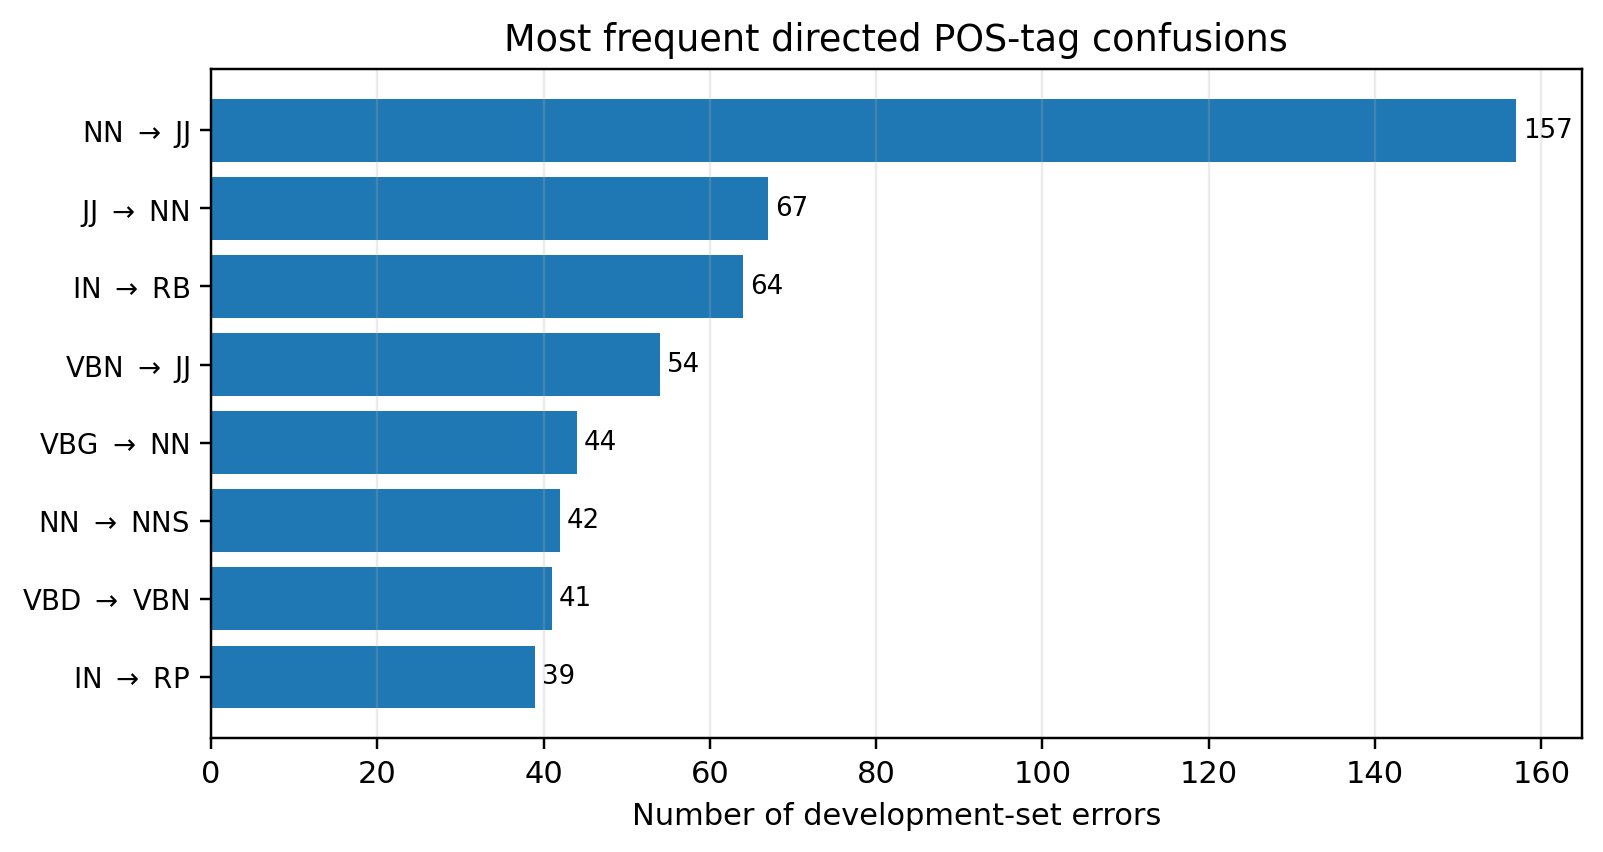
\includegraphics[width=\linewidth]{figures/dev_confusions.png}
\caption{Most frequent directed tag confusions on the provided development set.}
\label{fig:confusions}
\end{figure}

\section{Conclusion and Limitations}
Under the PA2 constraints, a trainable 100-D word/character/shape representation followed by a BiLSTM is a strong compact solution. Character information provides the clearest gain: it substantially improves overall and OOV validation accuracy over a word-only model. Bidirectional context is also important, while CNN versus character LSTM and softmax versus CRF yield only small single-run accuracy differences; the CNN/softmax path offers a favorable runtime trade-off. Label smoothing is the best single-run validation configuration, but its validation OOV accuracy is lower than the unsmoothed full model, which motivates a targeted multi-seed check before making a strong claim.

The experiment search used one seed, so close rankings may reflect initialization or data-split variance. The development corpus is not the blind test set, and the 97.739\% score should not be described as blind-test accuracy. Adarsh’s independently built HMM aggregate result remains pending. The standalone neural build runtime was not separately measured; the reported 132.6 s is the measured full-data refit within the complete experiment pipeline, not a standalone builder measurement. A token-by-token HMM comparison requires its aligned prediction file. The no-pretrained-vector rule rules out using GloVe, Word2Vec, BERT, or RoBERTa vectors as a direct replacement for the learned embeddings.

\bibliographystyle{acl_natbib}
\bibliography{references}
\end{document}
